\documentclass{article}
\usepackage[utf8]{inputenc}
\usepackage[numbers]{natbib}
\usepackage{amsmath}
\usepackage{url}
\usepackage{graphicx}
\usepackage{floatrow}
\usepackage{pdfpages}
\usepackage{csvsimple}
\usepackage{tikz}
\usepackage{pgfplots}
\usepackage{filecontents}

\author{Joris Damian Morger, Nicolas Manuel Alessandro Gagliani, IT12T}

\title{Zweikörpersysteme - Auftrag PSIT HS 2013}

\begin{document}
	\maketitle

	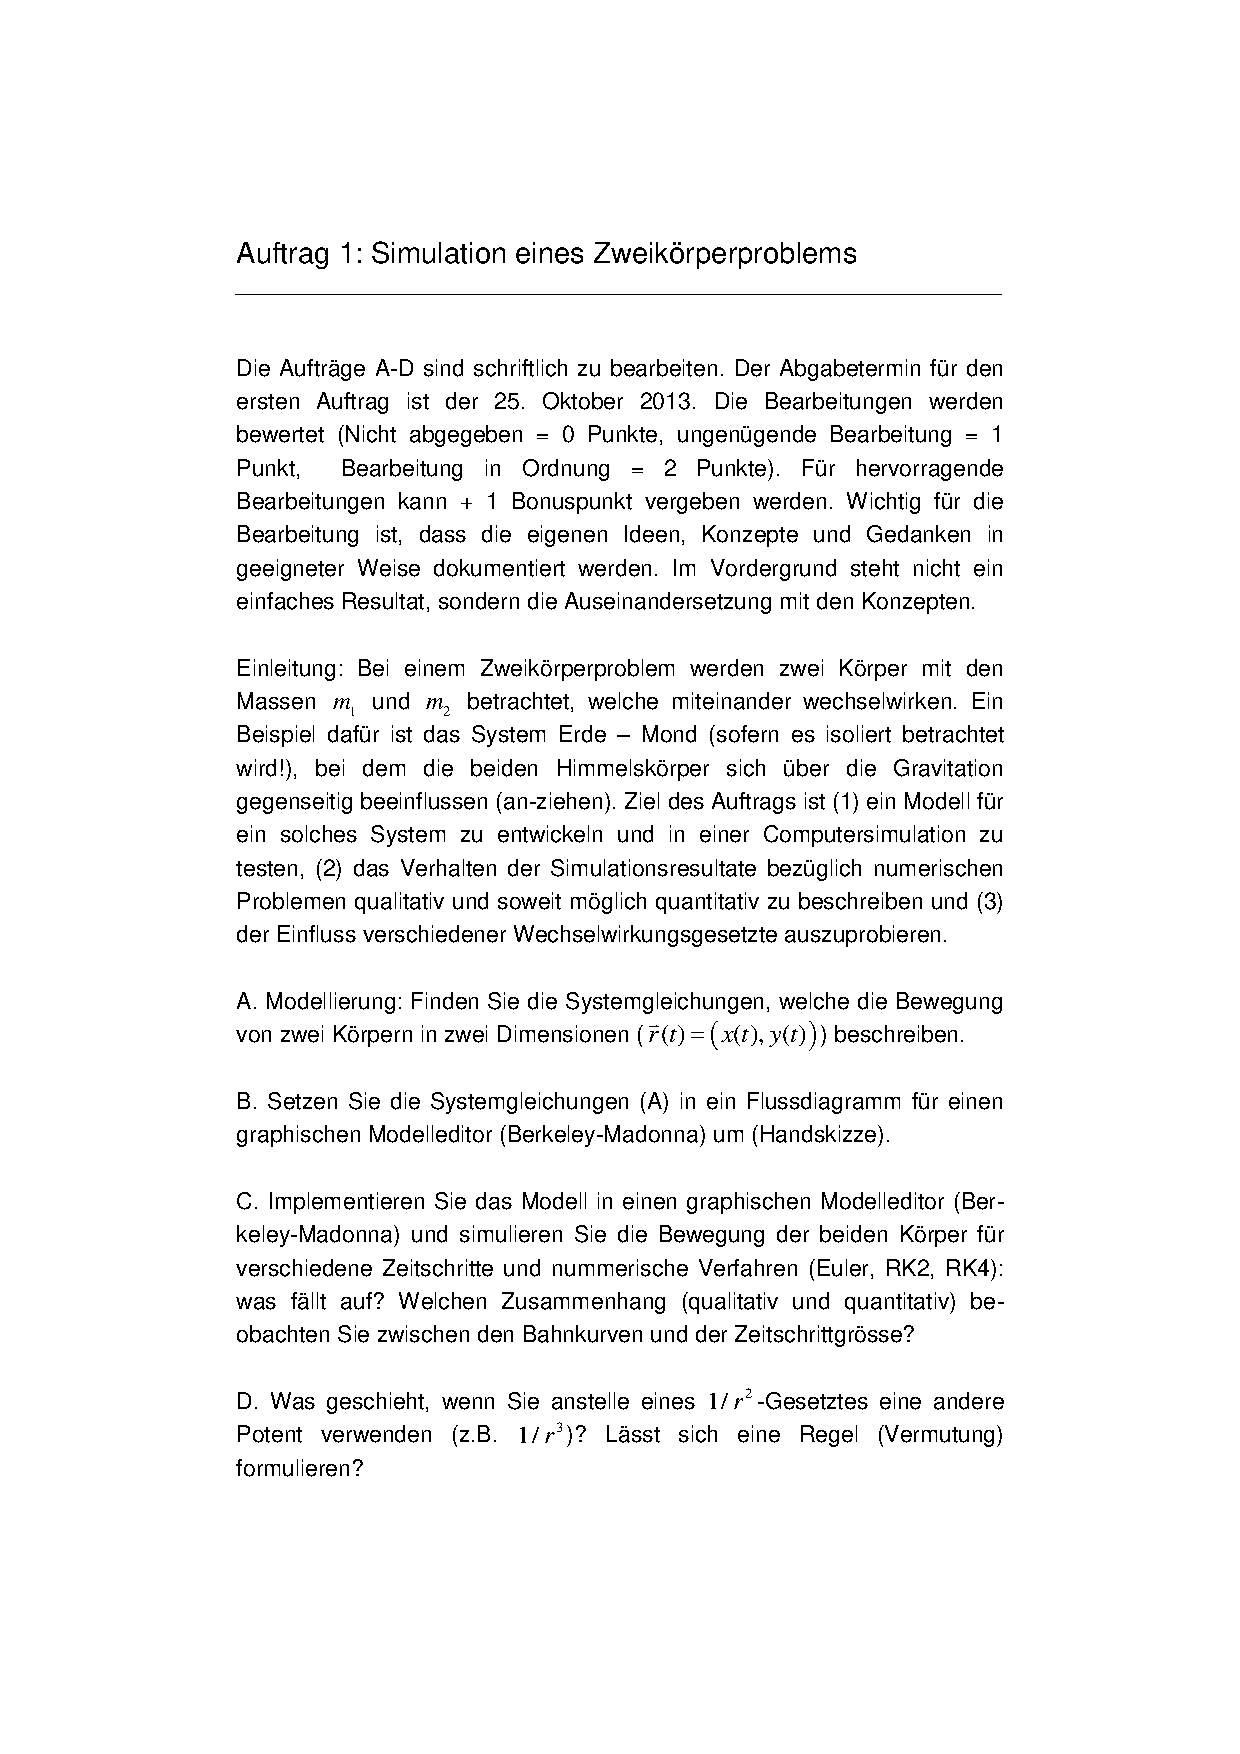
\includepdf[pages={1}]{PhITAuftr1.pdf}

	\section*{Intro}

	Wir betrachten im folgenden zwei isolierte Körper Erde und Mond mit den Massen $m_{Mond}$ und $M_{Erde}$, wobei der Mond in ellipsenförmig um die Erde rotiert.
	\par
	\bigskip
	Per Definition:
	$$m_{\text{M}} = 7.35 \times 10^{22} \text{ kg} \cite{wiki1}$$

	$$m_{\text{E}} = 5.79 \times 10^{24} \text{ kg} \cite{wiki1}$$

	$$r_{\text{ME}} (Abstand) = 3,844 \cdot 10^8 \text{ m} \cite{wiki2}$$

	$$\gamma = 6.6742^{-11} \frac{Nm^{2} }{kg^2 }$$


	\section*{Teil A}
	\subsection{Gravitationskraft}
	Erde und Mond ziehen sich an. Die Kraft zwischen den beiden Massen lässt sich wie folgt berechnen:

	Wir wissen:

	$$T = 27,3217d \approx 2360594s$$
	$$\omega = \frac{2\pi}{T}$$
	$$F_{Z} = m\omega^2r$$

	Daher:
	$$\omega_\text{M} = \frac{2\pi}{T} = \frac{2\pi}{27,3217d} = \frac{2\pi}{2360594s} \approx 2.66\cdot10^{-6} s^{-1}$$
	$$F_\text{Z} = m_\text{M} \cdot \omega_\text{M}^2 \cdot r_\text{ME} \approx 2 \cdot 10^{20} N$$

	$$F_{G,M} = \gamma \cdot \frac{{m_\text{E} \cdot m_{\text{M}}}}{{{|{\vec{r_{ME}}}}|^2}}} \cdot \vec{n} \approx -2 \cdot 10^{20} N$$

	Aha! Da die Zentripedalkraft vom Mond und die Gravitationskraft zwischen Mond und Erde die gleiche ist, einfach mit anderem Vorzeichen (also Kraft in andere Richtung), erkennen wir das der Mond und die Erde sich in Balance halten. Sie prallen weder aufeinander, noch bewegen sie sich voneinander weg.

	Bisher haben wir vernachlässigt das der Radius vom Mond zur Erde nicht immer gleich gross ist, da die Erde sich auch noch um eine Achse dreht.

	\begin{figure}[h!]
			\caption{Radius verändert sich}
		    \centering
			    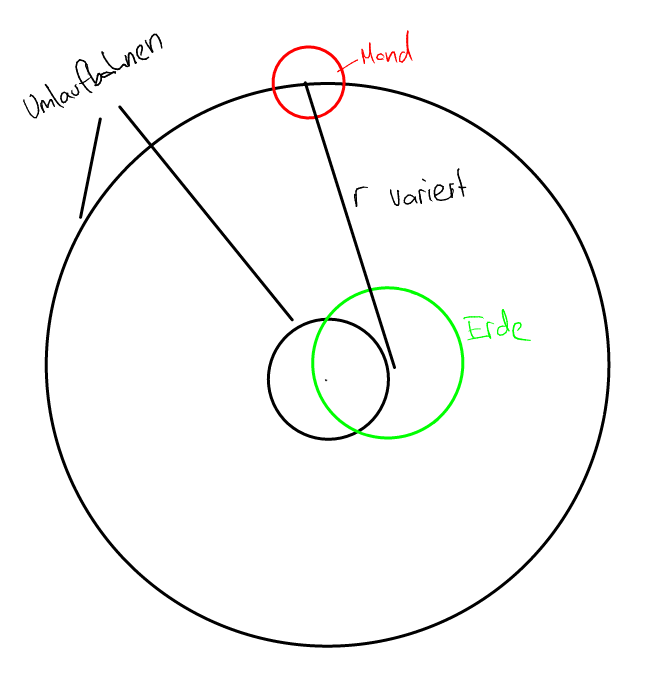
\includegraphics[width=0.5\textwidth]{radius}
	\end{figure}


	Daher müssen wir eine Funktion finden die den Radius zwischen Mond und Erde genauer beschreibt.

	Wir wissen der Massenmittelpunkt zwischen Erde und Mond ist
		$$ r_\text{T} = \frac{r_\text{M}}{r_\text{E}} = \frac{1}{81} = 4'683 \text{km} $$

	% \includegraphics*[100,100][300,300]{situationsskizze}


	\section*{Teil B}
	\begin{tikzpicture}
		\begin{axis}[
			width=15cm, height=8cm,     % size of the image
			grid = major,
			grid style={dashed, gray!30},
			xmin=-600000000,     % start the diagram at this x-coordinate
			xmax=600000000,    % end   the diagram at this x-coordinate
			ymin=-400000000,     % start the diagram at this y-coordinate
			ymax=400000000,   % end   the diagram at this y-coordinate
			ylabel=test,
			xlabel=moon,
			]

		\end{axis}
	\end{tikzpicture}

	Eigentlich hatten wir die Lösung schon längst in Berkeley Madonna, haben aber die längste Zeit nach einem Fehler gesucht der eigentlich keiner war. Das Problem war das wir im Parameter Window zu wenige Zeitschritte gemacht haben und zu früh aufgehört haben. So haben wir nie gesehen wie die eigentliche Kurve sich entwickelt hat. 
	\section*{Teil C}
	\section*{Teil D}

	\bibliographystyle{ieeetr}
	\bibliography{auftrag}
\end{document}

